\documentclass[letterpaper,12pt]{article}
%\usepackage{harvard}
%\usepackage{subfigure}
%\usepackage[active]{srcltx}
\usepackage{graphicx}
\usepackage{pdflscape}
\usepackage{amsmath}
\usepackage{amsthm}
\usepackage{lscape}
\usepackage{enumerate}
\usepackage{float}
\usepackage{grffile}
\usepackage{relsize}
\usepackage{tablefootnote}
\usepackage{footnote}
\usepackage{sectsty}
\usepackage{xcolor}
\usepackage{caption}
\usepackage{color}
\usepackage{natbib}
\usepackage{multirow}
\usepackage{bbm}
\usepackage[T1]{fontenc}
\usepackage[multiple]{footmisc}
\usepackage{appendix}
\usepackage{times}
\usepackage{relsize}
\usepackage{caption}
\usepackage{newtxtext,newtxmath}
\usepackage{enumitem}


%%%%%%%%%%%%%%%%%%%%%%%%%%%%%%%%%%%%%%%%%%%%%%%%%%%%%%%%%%%%
%%%   Title Page Information
%%%%%%%%%%%%%%%%%%%%%%%%%%%%%%%%%%%%%%%%%%%%%%%%%%%%%%%%%%%%
\title{\vspace{-1in}ECON311, Winter 2025: Final Exam}
\author{Leandro Freylejer}
\date{}

%%%%%%%%%%%%%%%%%%%%%%%%%%%%%%%%%%%%%%%%%%%%%%%%%%%%%%%%%%%%
%%%   Double and Single Space Commands
%%%%%%%%%%%%%%%%%%%%%%%%%%%%%%%%%%%%%%%%%%%%%%%%%%%%%%%%%%%%
\newlength{\defbaselineskip}
\setlength{\defbaselineskip}{\baselineskip}
\newcommand{\setlinespacing}[1]{\setlength{\baselineskip}{#1 \defbaselineskip}}
\newcommand{\doublespacing}{\setlength{\baselineskip}{1.3 \defbaselineskip}}
\newcommand{\singlespacing}{\setlength{\baselineskip}{1\defbaselineskip}}
\renewcommand{\thesubsection}{\arabic{subsection}}
\newtheoremstyle{dotlessS}{}{}{\itshape}{}{\color{dg}\bfseries}{}{ }{}
\theoremstyle{dotlessS}
\newtheorem{theorem}{Theorem}
\newtheorem{lemma}{Lemma}
\newtheorem{proposition}{Proposition}
\newtheorem{assumption}[theorem]{Assumption}
\newtheorem{corollary}{Corollary}
\newtheorem{definition}{Definition}
\newenvironment{example}[1][Example]{\begin{trivlist}
\item[\hskip \labelsep {\bfseries #1}]}{\end{trivlist}}
\newenvironment{remark}[1][Remark]{\begin{trivlist}
\item[\hskip \labelsep {\bfseries #1}]}{\end{trivlist}}

\newcommand\Pitem{%
  \addtocounter{enumi}{-1}%
  \renewcommand\theenumi{\arabic{\enumi}'}%
  \item%
  \renewcommand\theenumi{\arabic{enumi}}%
}

%%%%%%%%%%%%%%%%%%%%%%%%%%%%%%%%%%%%%%%%%%%%%%%%%%%%%%%%%%%%
%%%   Set Margins Here
%%%%%%%%%%%%%%%%%%%%%%%%%%%%%%%%%%%%%%%%%%%%%%%%%%%%%%%%%
\textwidth=6.5in
\textheight=9in
\oddsidemargin=0.10in
\evensidemargin=0.10in
\topmargin=-0.5in
%\parskip=3pt

%%%%%%%%%%%%%%%%%%%%%%%%%%%%%%%%%%%%%%%%%%%%%%%%%%%%%%%%%%%%%
%%%   Actual Document Begins Here
%%%%%%%%%%%%%%%%%%%%%%%%%%%%%%%%%%%%%%%%%%%%%%%%%%%%%%%%%%%%%
\begin{document}
\pagenumbering{arabic}
\maketitle
\noindent There are two parts in this exam. Part I has five questions and Part II has two questions for a total of 87 points. You must show all your work to get full marks. You are allowed a calculator. Good Luck!!!
\section{Part I: Short-Answer Questions}

\subsection*{Question I}
Consider the following Romer economy: 
\begin{eqnarray*}
\begin{array}{ll}
\text{Production Function:} & Y_t=A_t  \: L_{Y_t} \\[1.4ex]
\text{Productivity:} & A_{t+1}=A_t+\overline{z} \: A_t \: L_{A_{t}}  \\[1.4ex]
\text{Allocation of labour:} & L_{A_{t}}=\overline{I} \: \overline{L}, \: \: \:  \: \: L_{Y_{t}}=(1-\overline{I}) \: \overline{L}  \\[1.4ex]
\end{array}
\end{eqnarray*}
\begin{enumerate}[label=(\alph*)]
\item (4 points) Derive the rate of growth of output per person in the long-run equilibrium ($g_y$)
\item (6 points) Use the previous equation to explain the trade-off between long-run growth and the short-run level of consumption in this model. In your answer make sure to include a graph with output per person on the vertical axis (using a ratio scale) and time on the horizontal axis. Label your graph carefully, including slopes.
\end{enumerate} 

\subsection*{Question II (4 points)}
Suppose that in a model, the law of motion for capital is given by: $K_{t+1}=\overline{s} \: Y_t+(1-\overline{d})K_{t}$. Using this Law of Motion, argue that in any Balance Growth Path Equilibrium (BGP) the following holds: $g_Y=g_K$ [Hint: to answer this question you need to remember that all variables grow at a constant rate in a BGP]

\subsection*{Question III (6 points)}
Using the IS-MP model carefully explain the impact on output and inflation of a permanent $TFP$ ($\overline{A}$) shock (i.e. a permanent supply-side shock). As in class, you may assume that the shock affects short- and long-run parameters equally, but that the government is initially not aware of the shock. In your discussion, make sure to show how the IS and Phillips Curves shift as well as an explanation of output overshooting in the short run. Label all your graphs carefully.

\newpage 

\subsection*{Question IV (6 points)}
Refer to Figure 1, where c refers to consumption per worker and y to output per worker, when answering the following question.
\begin{figure}[H]
\centering
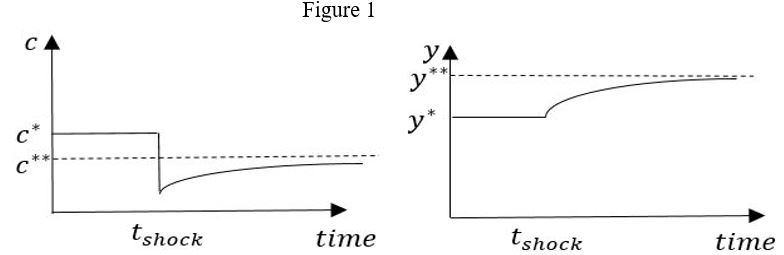
\includegraphics[scale=.75]{Solow_model}
\end{figure}
Consider the Solow Model economy studied in class:
\begin{eqnarray*}
\begin{array}{ll}
\text{Production Function} &Y_t=\overline{A} \: \left(K_t\right)^{\frac{1}{3}} \: \left(\overline{L}\right)^{\frac{2}{3}}\\[1.4ex]
\text{Capital Accumulation} &K_{t+1}=I_t+(1-\overline{d}) \: K_t \\[1.4ex]
\text{Resource Constraint} &C_t+I_t=Y_t  \\[1.4ex]
\text{Allocation of Resources} &I_t=\overline{s} \: Y_t  \\[1.4ex]
\end{array}
\end{eqnarray*}
Use this model to show the shock at time $t_{shock}$ that best describes the transitional dynamics in Figure 1. To answer this question use the Solow diagram with total output.

\subsection*{Question V (6 points)}
Suppose that the IS curve is as follows: $\widetilde{Y}_t=\frac{1}{1-b_c} \: [\overline{a}-\overline{b}_i \: (R_t-\overline{r})]-1$, $R_t=R^{ff}_t+\overline{f}$ and that the Phillips Curve is as follows: $\Delta \pi_t=\overline{v}\widetilde{Y}_t+\overline{o}_t$ . Suppose that the economy starts at its long-run equilibrium with no financial frictions ($\overline{a}=(1-b_c)$, $\overline{f}=0$, $\overline{o}_t=0$), use the IS-MP and Phillips Curve to show what happens to this economy if it experiences a negative demand shock and a concurrent increase in risk ($\overline{f}$) --- i.e. show what happens to the economy when there is a financial crisis. For this question, you may assume no monetary policy response to the crisis. 

\section{Part II: Long-Answer Questions}



\section*{Question I: The AS-AD Model}
Consider the following economy:
\begin{eqnarray*}
\begin{array}{ll}
\text{IS- Curve} & \widetilde{Y}_t=\frac{1}{1-b_c}\left[\overline{a}-\overline{b}_i \: (R_t-\overline{r})\right]-1 \\[1.4ex]
\text{Inflation} & \pi_t=\pi^e_t+\overline{v} \: \: \: \widetilde{Y}_t+\overline{o}_t, \: \: \pi^e_t=\pi_{t-1}  \\[1.4ex]
\text{Policy Rule} & R_t-\overline{r}=\overline{m}(\pi_t-\overline{\pi})  \\[1.4ex]
\end{array}
\end{eqnarray*}
Use the previous equations to answer the following questions:
\begin{enumerate}[label=(\alph*)]
\item (3 points) Derive the AD curve.
\item (10 points) With all the economic uncertainty introduced by Donald Trump's economic policies, there has been a loss in consumer and investor confidence. Concurrently, the increase in tariffs, in particular the large increase in tariffs on Chinese made products, has resulted in a large inflation shock. Suppose that the economy starts at its long-run equilibrium and that the loss of confidence results in a multi-period negative demand shock, while the tariffs results in a one-time cost shock. Using the AS-AD model, carefully explain what happens to the economy immediately following these shocks and over time. You may assume that the negative demand shock lasts \textbf{many} periods, and that the resulting inflation in the period of the cost shock is above the Federal Reserve target level ---[This gives you information on the location of the AS curve in the period of the cost shock and the period immediately after the cost shock].
\item (5 points) Is the initial recession better or worse than without the inflation shock. Explain.
\end{enumerate}


\section*{Question II: IS-MP Model}
Consider the following economy:
\begin{eqnarray*}
\begin{array}{ll}
\text{Expenditure:} & E_t=C_t+I_t+G_t+X_t-M_t \\[1.4ex]
\text{Consumption:} &C_t=a_c+b_c (Y_t-T_t) \\[1.4ex]
\text{Investment:} & I_t=a_i -b_i \: \: \: R_t \\[1.4ex]
\text{Imports:} & M_t=b_m \: \: \: Y_t  \\[1.4ex]
\text{Inflation:} & \pi_t=\pi_{t-1}+\overline{v} \: \: \: \widetilde{Y}_t+\overline{o}_t  \\[1.4ex]
\text{Exogenous Variables:} & G_t=\overline{G}, \: \: \: \: \: \: T_t=\overline{T}, \: \: \: \: \: \: X_t=\overline{X}
\end{array}
\end{eqnarray*}
, where $0<b_m<1$ and $0<b_c<1$. In this economy, imports depend on the level of income. Moreover, consumption depends on disposable income (income net of taxes) and not just on the level of income as we previously assumed (taxes are exogenous in this economy). Use the previous equations to answer the following questions:
\begin{enumerate}[label=(\alph*)]
\item (7 points) Solve for the equilibrium in the goods market. What is the expenditure multiplier? 
\item (7 points) Use the Keynesian Cross to carefully explain the effect of an exogenous increase in taxes ($\overline{T}$) (carefully label the graph). What is the assumption we need to make to guarantee that an equilibrium exists? Explain.
\item (6 points) Derive the IS curve using deviations from potential output as the endogenous variable.
\item (10 points) Suppose the economy is at its potential output equilibrium with a constant $2\%$ inflation rate. Assume that in the year 2000 there is a negative demand shock lasting until 2001 and decreasing the inflation rate by $1$ percentage points per year (this is a two-year recession). Assume that in 2004 the government decides to use monetary policy to increase  inflation back to its $2\%$ level by increasing output above its potential level by the same amount for two consecutive years. Using the full short-run model (IS-MP and Phillips curve), explain what happens to the economy \textbf{over time}. Be sure to include graphs showing how output and inflation respond over time (carefully label all graphs).
\item (7 points) Net exports, denoted by $NX_t=\overline{X}-M_t$, model the economy's foreign trade. A positive value of $NX_t$ denotes a trade surplus and a negative value denotes a trade deficit. Suppose that the economy is in its long-run equilibrium when trade is balanced ($NX=\overline{X}-b_m \: \: \: \overline{Y}=0$), using a graph with $NX$ in the vertical axis and time on the horizontal axis show what happens to $NX_t$ from 1999 onwards.
\end{enumerate}   

\end{document}